\begin{frame}\frametitle{Long Baseline Neutrino Facility (LBNF) Experimental Setup}
\scriptsize
\begin{figure}
\label{fig:LBNF_overallScheme}
\centering
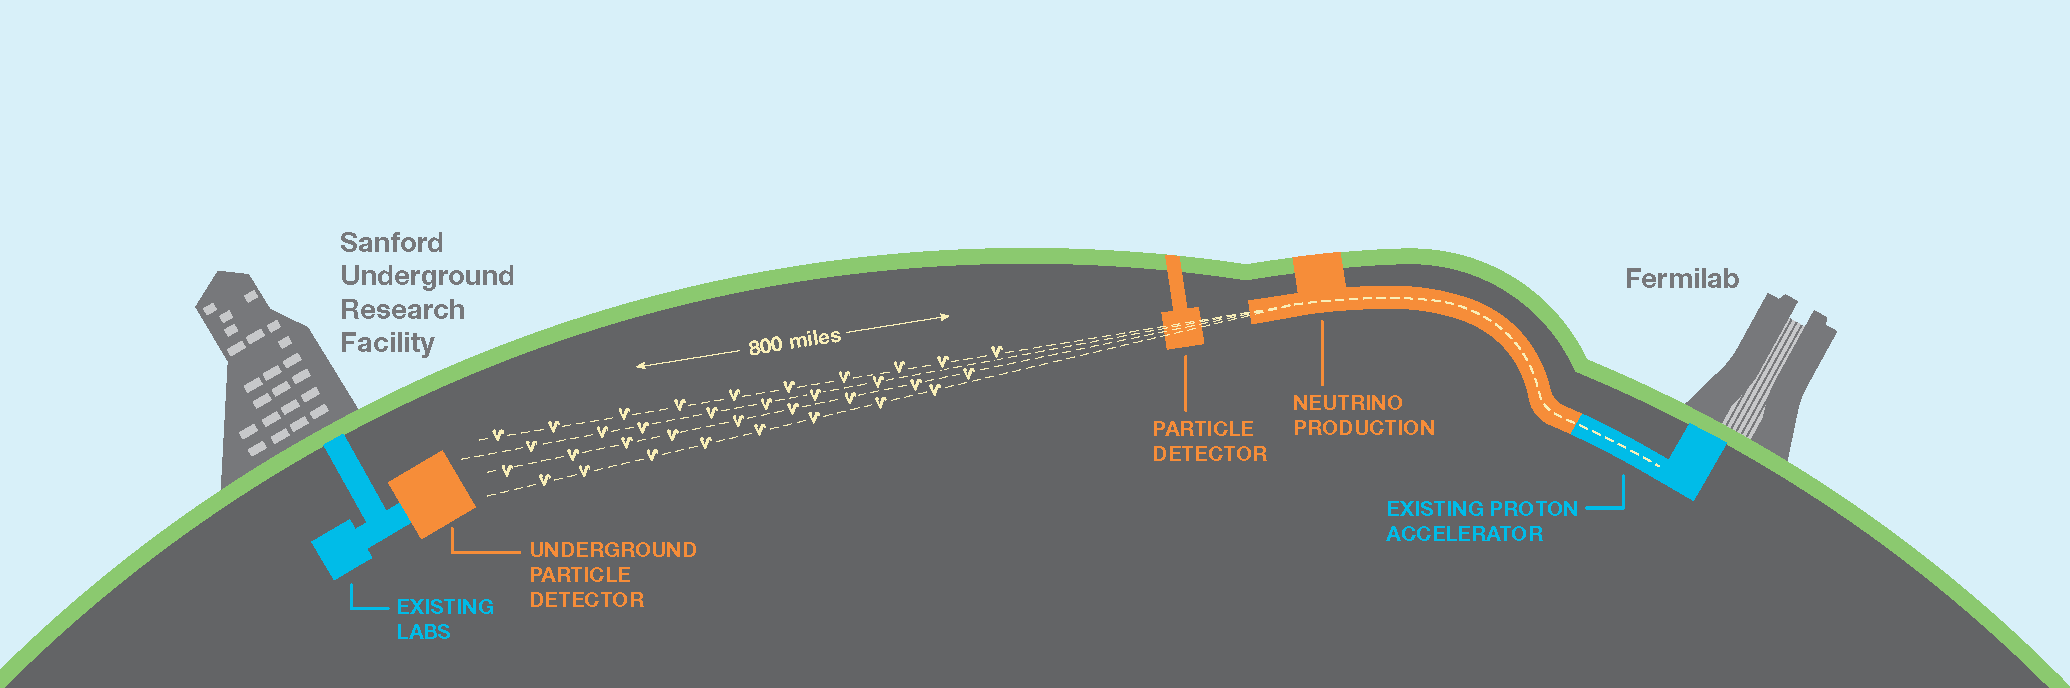
\includegraphics[width=0.95\textwidth, keepaspectratio=true]{figs/LBNF_overallScheme.png} 
\end{figure}
\begin{itemize}
  \item neutrino beam production system at FNAL, Illinois 
  \item near detector at FNAL, Illinois 
  \item far detector at SURF, South Dakota
\end{itemize}
\tiny
FNAL - Fermilab National Accelerator Laboratory, SURF - Sanford Underground Research Facility\\
Source of figure: \cite{ref_LBNFweb} 
\end{frame}

\begin{frame}\frametitle{$P(\nu_\mu \rightarrow \nu_e)$ at a baseline of 1300 km}
  \scriptsize
  \begin{figure}
  \label{fig:LBNF_oscProbability}
  \centering
  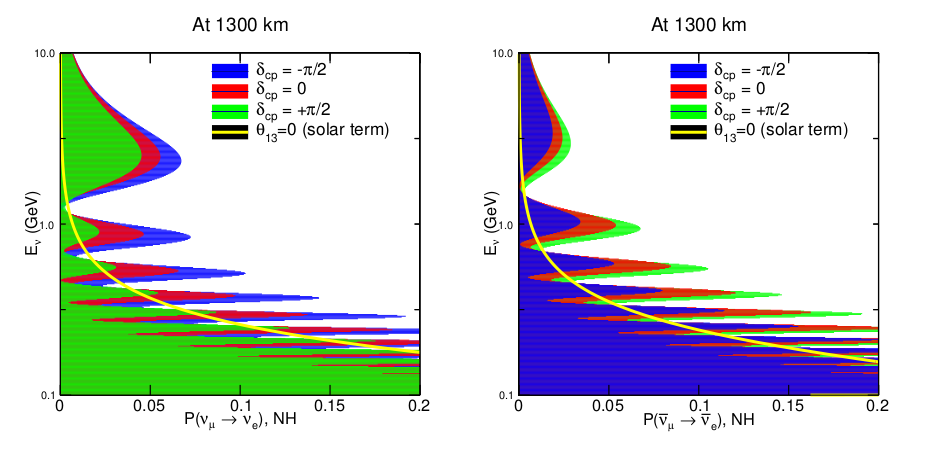
\includegraphics[width=0.98\textwidth, keepaspectratio=true]{figs/LBNF_oscProbability.png}
  \\$P(\nu_\mu \rightarrow \nu_e)$ at a baseline of 1300 km (as LBNF will have), as a function of neutrino energy. Left - neutrinos, right - antineutrinos. Source of figure: LBNF CDR draft, volume physics \cite{ref_LBNFdoc_volume-physics}
  \end{figure}
\end{frame}

\begin{frame}\frametitle{LBNF. Beam Production System}
\scriptsize
\begin{figure}
\label{fig:LBNF_nuBeam}
\centering
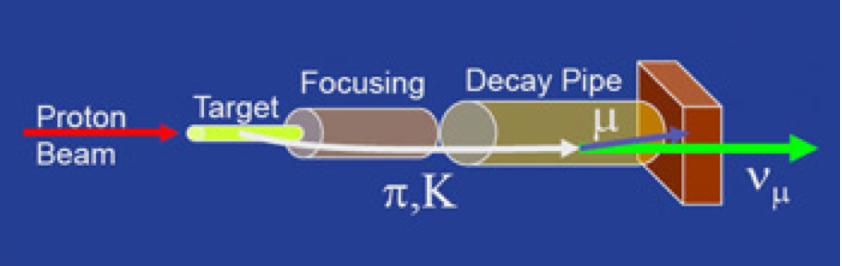
\includegraphics[width=0.65\textwidth, keepaspectratio=true]{figs/LBNF_nuBeam.png}  
\end{figure}
The neutrino beam production at the LBNF. Source of figure: \cite{ref_LBNFweb}\\
\begin{itemize}
  \item Proton beam from Fermilab accelerator hits target
  \item Protons scatter on target atoms and produce pions and kaons {\tiny (more details on the next slide)}
  \item Charged pions and kaons are focused
  \item And decay in the decay pipe, producing muon neutrino beam
  \item Neutrinos are registered by near detector, $\sim 200$ m away from the target
  \item And by far detector, $\sim 1300$ km away from the target
\end{itemize}
\end{frame}

\begin{frame}\frametitle{LBNF. Feynmann diagrams of pions and kaons production and decay}
\scriptsize
\begin{figure}
\label{fig:pionAndKaonProductions}
\centering
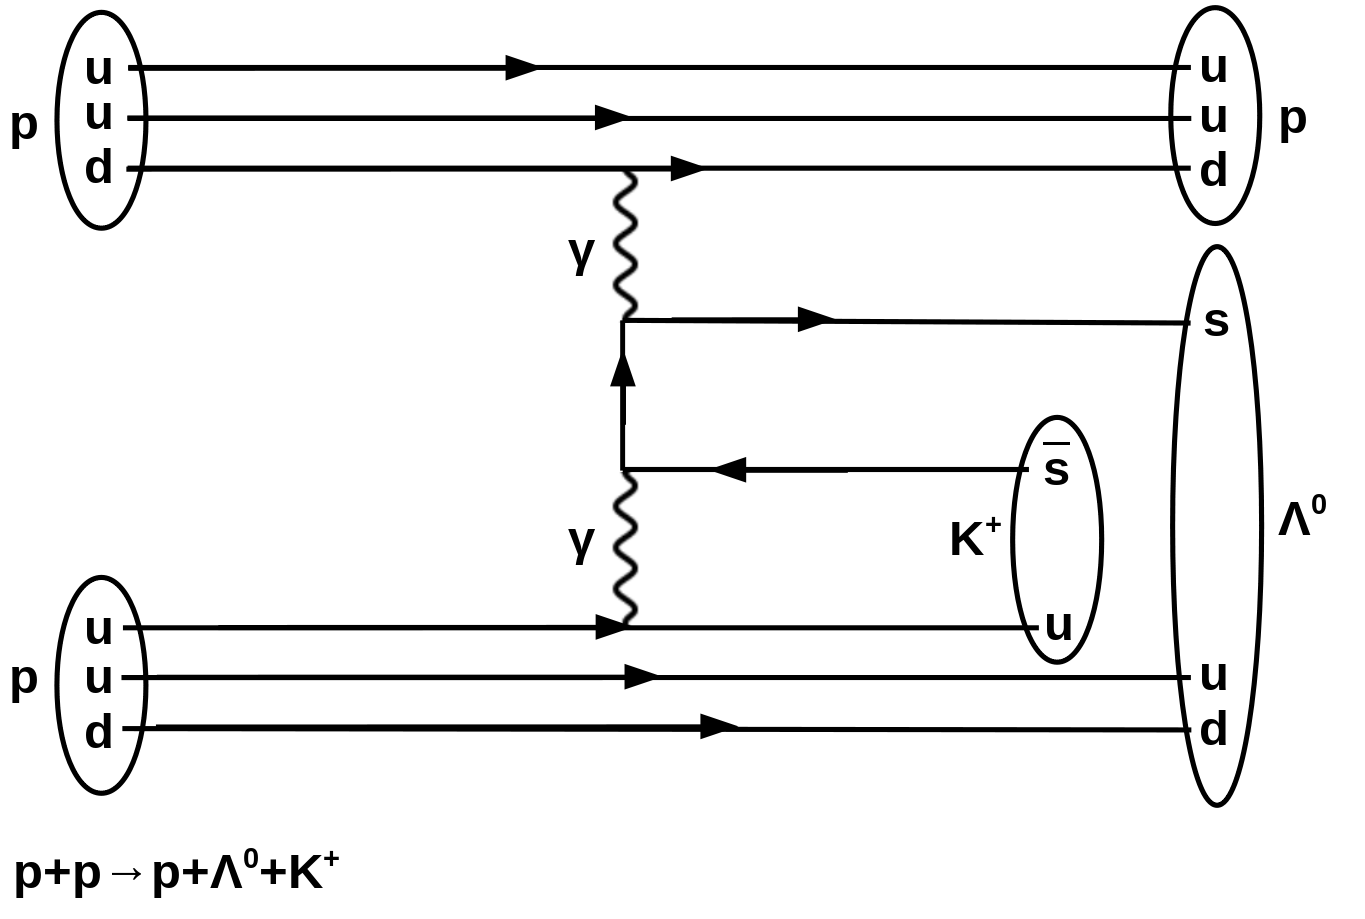
\includegraphics[width=0.48\textwidth, keepaspectratio=true]{figs/ppKaonProduction.png}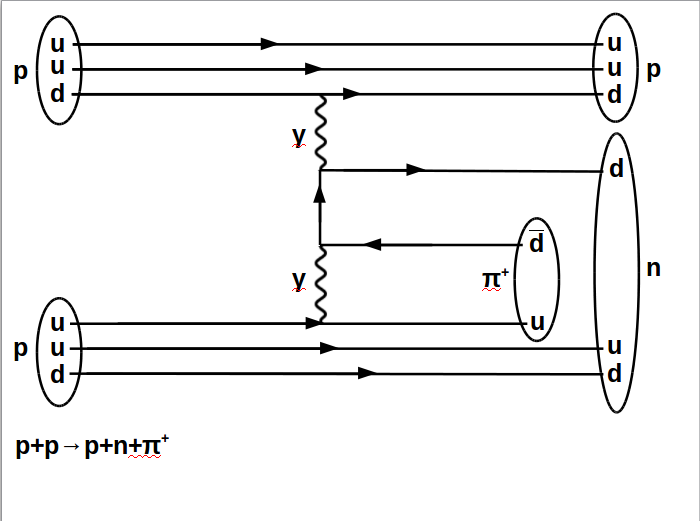
\includegraphics[width=0.48\textwidth, keepaspectratio=true]{figs/ppPionProduction.png}  
\end{figure}
\begin{figure}
\label{fig:pionAndKaonDecays}
\centering
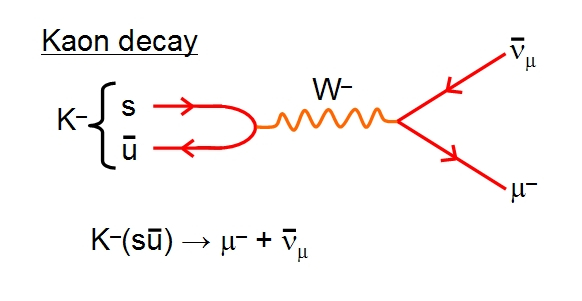
\includegraphics[width=0.45\textwidth, keepaspectratio=true]{figs/kaonDecay.jpg}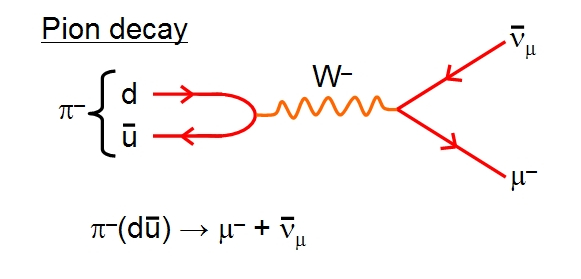
\includegraphics[width=0.45\textwidth, keepaspectratio=true]{figs/pionDecay.jpg} 
\end{figure}
\tiny Source of bottom figure \cite{ref_fig_pionandKaonDecays}.
\end{frame}

\begin{frame}\frametitle{LBNF. Near Detector Cavern}
\scriptsize
\begin{figure}
\label{fig:nearDetector}
\centering
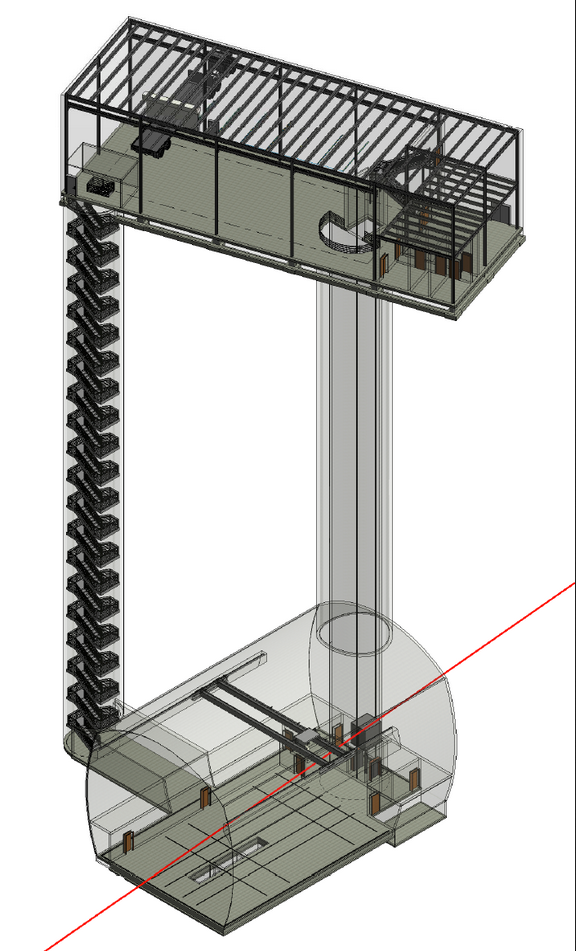
\includegraphics[width=0.35\textwidth, keepaspectratio=true]{figs/nearDetector_project.png}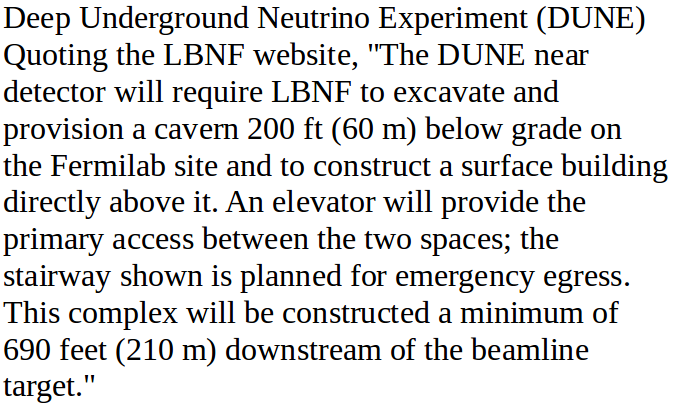
\includegraphics[width=0.55\textwidth, keepaspectratio=true]{figs/nearDetector_Text.png}
\end{figure}
%\scriptsize
%Deep Underground Neutrino Experiment (DUNE)
%Quoting the LBNF website \cite{ref_LBNFweb}, "The DUNE near detector will require LBNF to excavate and provision a cavern 200 ft (60 m) below grade on the Fermilab site and to construct a surface building directly above it. An elevator will provide the primary access between the two spaces; the stairway shown is planned for emergency egress. This complex will be constructed a minimum of 690 feet (210 m) downstream of the beamline target."
\end{frame}

\begin{frame}\frametitle{LBNF. Near Detector}
\scriptsize
\begin{figure}
\label{fig:nearDetector}
\centering
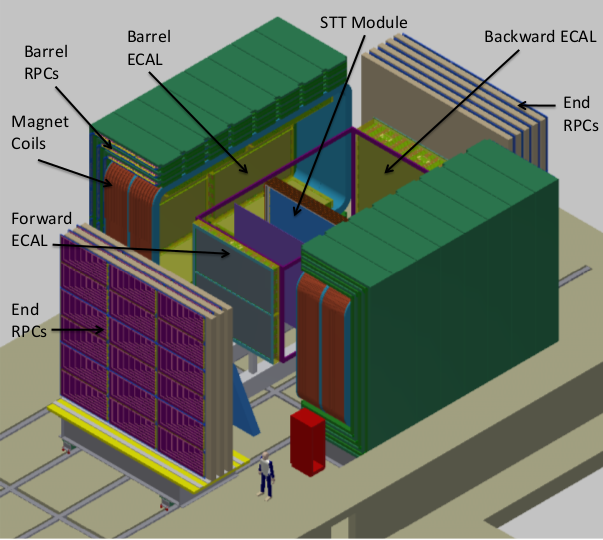
\includegraphics[width=0.50\textwidth, keepaspectratio=true]{figs/nearDetector.png}
\end{figure}
\scriptsize
The detector will consist of central Straw-Tube Tracker (STT) modules, electromagnetic calorimeter (ECAL), magnet coils of 0.4T and muon identification system consisting of Resistive Plate Chamber (RPC) modules. The neutrinos would come from the bottom left corner of the picture, to the End RPCs.\\
\end{frame}


\begin{frame}\frametitle{LBNF. SURF (Far Detector Site)}
\begin{figure}
\label{fig:farDetector_SURF1}
\centering
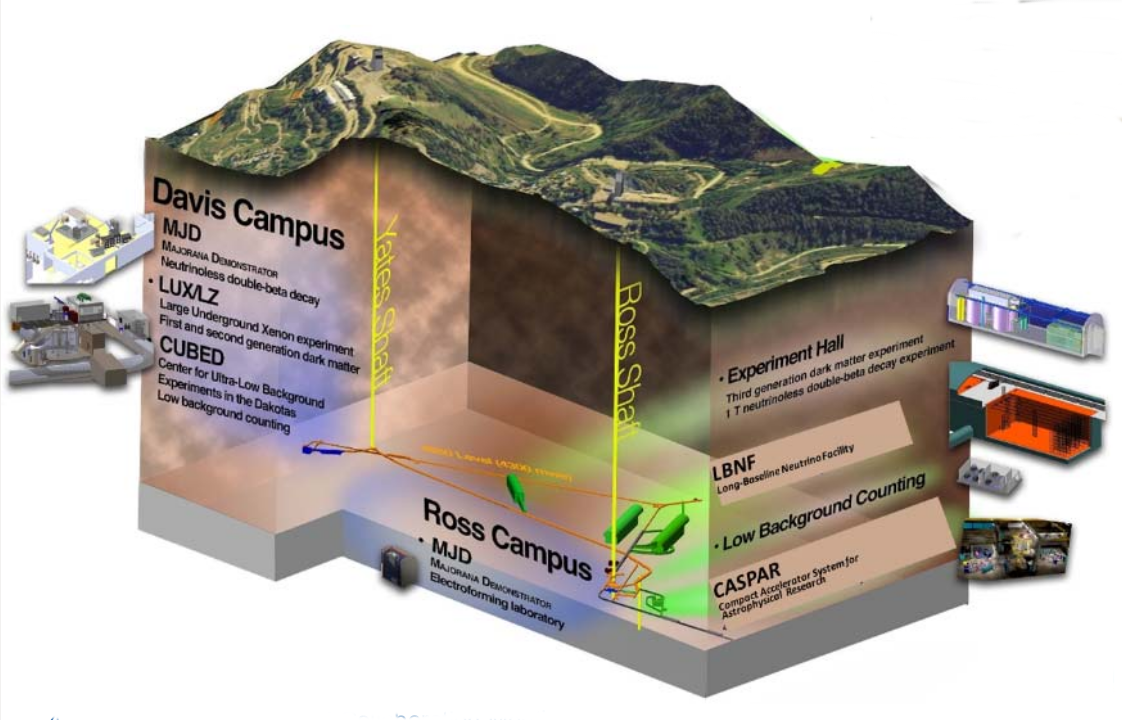
\includegraphics[width=0.98\textwidth, keepaspectratio=true]{figs/farDetector_SanfordUndergroundResearchFacility.png}
\end{figure}
\end{frame}

\begin{frame}\frametitle{LBNF. SURF (Far Detector Site)}
\begin{figure}
\label{fig:farDetector_SURF2}
\centering
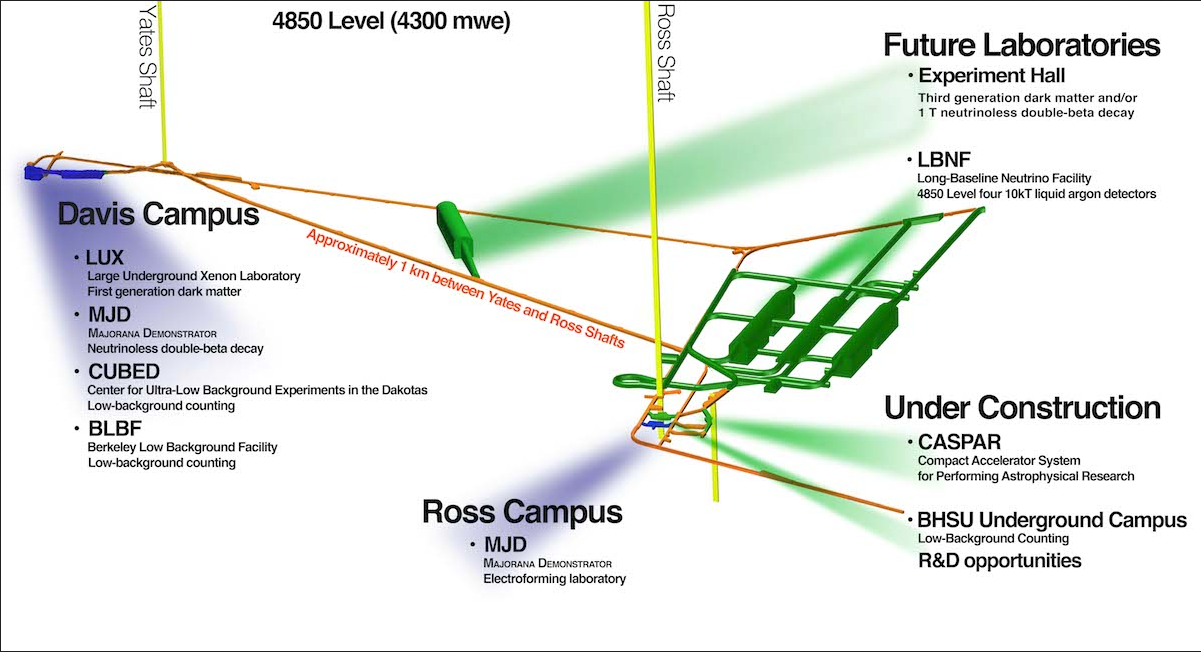
\includegraphics[width=0.98\textwidth, keepaspectratio=true]{figs/farDetector_wholeLab.png}
\end{figure}
\scriptsize
4 modules (15m x 12m x 58m, 10,000 tonnes of liquid argon each) placed into 4 caverns 1500 m underground. 5th cavern between two pairs - cryogenic equipment\\
\end{frame}

\begin{frame}\frametitle{LBNF. Far Detector. Liquid Argon Time Projection Chamber}
\begin{figure}
\label{fig:farDetector_TPC}
\centering
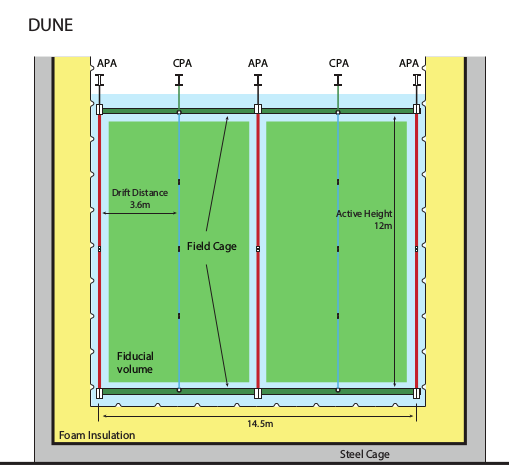
\includegraphics[width=0.75\textwidth, keepaspectratio=true]{figs/farDetector_TPC.png}
\end{figure}
\end{frame}

\begin{frame}\frametitle{LBNF Compared to the Other Experiments \cite{ref_LBN_OscExpReview}}
\tiny
  \begin{tabular}{|c|c|c|c|c|c|}
              & KEK (K2K) & NuMI & CNGS & T2K & LBNF (DUNE)\\ \hline
     location & Japan  & Illinois - & Switzerland - & Japan & Illinois - \\ 
              &        & Minnesota & Italy &  & South Dakota\\ \hline
     accelerator & KEK PS  & FNAL & CERN's SPS & J-PARC & FNAL\\ \hline
     time of oper. & 1999-2004  & 2005-2012 & 2006-2012 & 2010- & future \\ \hline 
     beam power  &  5 kW  & 300-350 kW  & 300 kW & 750 kW & 2000 kW\\ \hline 
     $E_p$  & 12 GeV & 120 GeV & 400 GeV & 30 GeV & 60-120 GeV\\ \hline 
     baseline  & 250 km & 735 km & 730 km & 295 km & 1300 km\\ \hline 
%                & KEK (K2K)   & NuMI                & CNGS                & T2K         & LBNF (DUNE)\\ \hline
     near        & (water ChD) & MINOS               & (muon               & ND280       & DUNE (FGD)\\  
     detector(s) & (FGD)       & (track. and scint.) & detector)           & INGRID      & \\ \hline 
     ND mass     & 1 kt (ChD)  & 0.98 kt             &                     &             & \\ \hline 
     far         & SuperK      & MINOS               & ICARUS (LAr)        & SuperK      & DUNE (LAr)\\  
     detector(s) & (water ChD) & track. and scint.   & OPERA (FGD)        & (water ChD) & \\ \hline 
     FD mass     & 50 kt       & 5.4 kt              & 0.76 kt (ICARUS)   & 50 kt       & 40 kt\\ 
                 &             &                     & 1.25 kt (OPERA)    &             & \\ \hline 
 \end{tabular}
\end{frame}
